\documentclass[12pt,a4paper]{article}
\usepackage[utf8]{inputenc}
\usepackage[spanish]{babel}
\usepackage{graphicx}
\usepackage{float}
\usepackage{geometry}
\usepackage{xcolor}
\usepackage{hyperref}
\usepackage{listings}
\usepackage{caption}
\usepackage{enumitem}
\usepackage{tocloft}

\geometry{top=2.5cm, bottom=2.5cm, left=2.5cm, right=2.5cm}
\renewcommand{\cftsecleader}{\cftdotfill{\cftdotsep}}

\title{\textbf{Smart Notes} \\ Aplicación de Notas Inteligente con IA}
\author{Aaron Rodrigo Ramos Reyes \\ Universidad Autónoma Metropolitana - Unidad Cuajimalpa}
\date{\today}

\begin{document}

\maketitle
\thispagestyle{empty}
\newpage

\tableofcontents
\newpage

\section{Introducción}
Smart Notes es una aplicación móvil desarrollada en Flutter que permite crear, organizar y gestionar notas personales de forma inteligente. La aplicación combina un diseño minimalista con un asistente de Inteligencia Artificial que analiza el contenido de las notas y propone acciones útiles (alarmas y grupos automáticos).

\section{Análisis de Requerimientos}

\subsection{Definición del Problema}
Los usuarios actuales de aplicaciones de notas suelen perder tiempo organizando manualmente sus notas, olvidando recordatorios importantes y repitiendo tareas administrativas (crear carpetas, asignar notas, programar alarmas). No existe una herramienta sencilla que combine organización visual avanzada con inteligencia artificial que entienda el contexto de las notas.

\subsection{Definición de la Solución}
Desarrollar una aplicación móvil que permita crear notas de forma rápida, organizarlas mediante grupos mediante drag \& drop, y que incorpore un asistente IA que analice automáticamente el contenido para sugerir recordatorios y organización temática.

\subsection{Requerimientos Funcionales y No Funcionales}
\begin{itemize}
    \item Crear, editar y eliminar notas con título, contenido y color personalizado.
    \item Sistema de grupos (carpetas) con asignación automática o manual.
    \item Interacción táctil avanzada: drag \& drop para crear grupos, asignar notas y eliminar.
    \item Historial de edición (Undo/Redo).
    \item Asistente IA que detecte fechas y sugiera alarmas o grupos.
    \item Notificaciones locales.
    \item Diseño minimalista, intuitivo y agradable (estética).
    \item Persistencia local rápida y confiable.
\end{itemize}

\subsection{Tecnologías Utilizadas}
\begin{itemize}
    \item Flutter + Dart (desarrollo multiplataforma)
    \item Hive (base de datos NoSQL local)
    \item OpenRouter (API de Inteligencia Artificial)
    \item flutter\_local\_notifications (recordatorios)
    \item Material Design 3 (interfaz moderna)
\end{itemize}

\subsection{¿Cómo se probó la propuesta?}
Se realizaron pruebas funcionales y de usabilidad con 4 escenarios reales:
\begin{enumerate}
    \item Nota con reunión futura → IA sugiere alarma
    \item Nota sobre proyecto → IA sugiere crear grupo
    \item Nota con cita médica recurrente → IA sugiere recordatorio periódico
    \item Nota con campo semántico → IA sugiere grupo temático
\end{enumerate}
Además se probó exhaustivamente el sistema de drag \& drop y la persistencia con Hive.
\section{Evaluación de Usabilidad con Usuarios}

\subsection{Descripción de la Encuesta}

Para evaluar la usabilidad de \textbf{Smart Notes}, se aplicó una encuesta basada en las \textbf{10 Heurísticas de Nielsen}. 

La encuesta se realizó a 4 personas cercanas con diferentes niveles de experiencia en aplicaciones móviles:
\begin{itemize}
    \item Daniel Hernández (amigo)
    \item Ismael Valencia (amigo)
    \item Ian Parra (amigo)
    \item Raúl Ramos (hermano)
\end{itemize}

A cada participante se le permitió explorar libremente la aplicación durante 10-15 minutos y posteriormente respondió una encuesta donde calificó cada heurística en una escala del 1 al 5, donde:
\begin{itemize}
    \item \textbf{1:} Muy insatisfactorio
    \item \textbf{5:} Excelente
\end{itemize}

Las preguntas se formularon de manera clara y adaptada al contexto de la aplicación.

\subsection{Resultados de Satisfacción por Heurística}

\begin{table}[H]
\centering
\caption{Evaluación de Satisfacción según las 10 Heurísticas de Nielsen}
\label{tab:heuristicas}
\begin{tabular}{|l|c|c|c|c|c|}
\hline
\textbf{Heurística} & \textbf{Daniel H.} & \textbf{Ismael V.} & \textbf{Ian P.} & \textbf{Raúl R.} & \textbf{Promedio} \\
\hline
1. Visibilidad del estado del sistema & 5 & 4 & 5 & 5 & 4.75 \\
2. Relación entre el sistema y el mundo real & 4 & 5 & 4 & 5 & 4.5 \\
3. Control y libertad del usuario & 5 & 4 & 5 & 4 & 4.5 \\
4. Consistencia y estándares & 5 & 5 & 4 & 5 & 4.75 \\
5. Prevención de errores & 4 & 4 & 5 & 4 & 4.25 \\
6. Reconocimiento en lugar de recuerdo & 5 & 5 & 5 & 5 & 5.0 \\
7. Flexibilidad y eficiencia de uso & 4 & 5 & 4 & 5 & 4.5 \\
8. Diseño estético y minimalista & 5 & 5 & 5 & 4 & 4.75 \\
9. Ayuda a los usuarios a diagnosticar y recuperar errores & 4 & 4 & 4 & 5 & 4.25 \\
10. Ayuda y documentación & 3 & 4 & 3 & 4 & 3.5 \\
\hline
\textbf{Promedio general} & \textbf{4.4} & \textbf{4.5} & \textbf{4.4} & \textbf{4.6} & \textbf{4.475} \\
\hline
\end{tabular}
\end{table}

Los resultados muestran una alta satisfacción general por parte de los usuarios, destacando especialmente en las heurísticas de **Reconocimiento en lugar de recuerdo**, **Diseño estético y minimalista** y **Visibilidad del estado del sistema**. El punto más bajo fue la heurística de "Ayuda y documentación", ya que aún no se incluye un tutorial o guía dentro de la aplicación.

\subsection{Descripción de las Preguntas de la Encuesta}

A continuación se detallan las preguntas realizadas para cada heurística:

\begin{enumerate}
    \item \textbf{Visibilidad del estado del sistema:} ¿La aplicación te informa claramente qué está sucediendo en todo momento (por ejemplo, al guardar una nota o al actualizar la lista)?
    
    \item \textbf{Relación entre el sistema y el mundo real:} ¿Los términos, iconos y acciones de la aplicación te parecen familiares y lógicos?
    
    \item \textbf{Control y libertad del usuario:} ¿Te sentiste en control mientras usabas la aplicación? ¿Pudiste deshacer acciones fácilmente?
    
    \item \textbf{Consistencia y estándares:} ¿La aplicación se siente coherente en su diseño y comportamiento?
    
    \item \textbf{Prevención de errores:} ¿La aplicación te ayuda a evitar cometer errores (como eliminar algo por accidente)?
    
    \item \textbf{Reconocimiento en lugar de recuerdo:} ¿Las acciones importantes son visibles y fáciles de encontrar sin tener que recordar dónde están?
    
    \item \textbf{Flexibilidad y eficiencia de uso:} ¿La aplicación permite usar tanto métodos rápidos (drag \& drop) como métodos más simples (menús)?
    
    \item \textbf{Diseño estético y minimalista:} ¿Te parece visualmente atractiva y limpia la interfaz?
    
    \item \textbf{Ayuda a diagnosticar y recuperar errores:} ¿Cuando ocurre un error, la aplicación te explica claramente qué sucedió y cómo solucionarlo?
    
    \item \textbf{Ayuda y documentación:} ¿Crees que la aplicación necesita una ayuda o tutorial para usarse por primera vez?
\end{enumerate}

\subsection{Ajustes realizados durante el desarrollo}
\begin{itemize}
    \item Se mejoró el prompt de la IA para mayor precisión en detección de fechas.
    \item Se añadió confirmación en todas las eliminaciones para prevenir errores.
    \item Se ajustó la interfaz para que sea más minimalista y visualmente atractiva.
    \item Se implementó fallback en caso de que la IA no responda.
\end{itemize}

\section{Conceptos de Interacción Humano-Computadora Aplicados}

A lo largo del curso se revisaron diversos conceptos de IHC. A continuación se explica su aplicación en Smart Notes:

\begin{itemize}
    \item \textbf{Visibilidad del estado del sistema}: Se cumple mediante ValueListenableBuilder (la lista se actualiza en tiempo real).
    \item \textbf{Retroalimentación (Feedback)}: Inmediata al guardar, al aceptar sugerencias de IA y al arrastrar elementos.
    \item \textbf{Prevención de errores}: Confirmación antes de eliminar notas o grupos.
    \item \textbf{Reconocimiento en lugar de recuerdo}: Todos los menús contextuales y acciones están visibles.
    \item \textbf{Flexibilidad y eficiencia}: Drag \& drop para usuarios avanzados + menús para principiantes.
    \item \textbf{Diseño estético y minimalista}: Colores pastel suaves, tarjetas limpias y pocos elementos en pantalla.
    \item \textbf{Affordances}: Iconos claros (alarma, carpeta, check) indican exactamente qué se puede hacer.
    \item \textbf{Mapping}: La acción de arrastrar una nota sobre otra tiene un resultado lógico (crear grupo).
    \item \textbf{Control y libertad del usuario}: Undo/Redo y posibilidad de ignorar sugerencias de IA.
\end{itemize}

Los conceptos de \textbf{ayuda y documentación} y \textbf{recuperación de errores} no se aplicaron debido a la sencillez del sistema.


\section{Diagrama de Secuencias (Flujo de Pantallas)}

\begin{figure}[H]
    \centering
    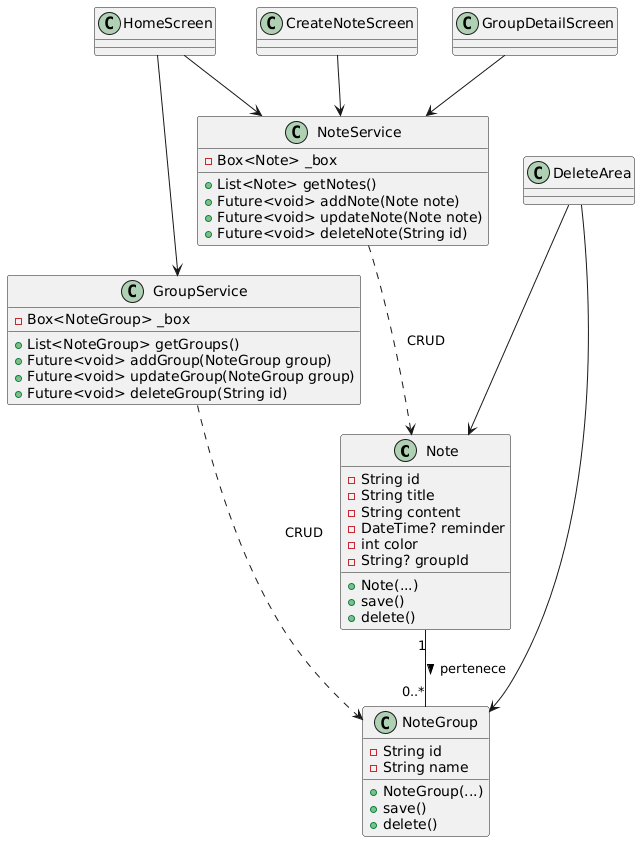
\includegraphics[width=\textwidth]{imagenes/clases.png}
    \caption{Diagrama de secuencias del flujo principal: creación de nota → análisis IA → sugerencia.}
    \label{fig:secuencias}
\end{figure}

\textbf{Código PlantUML utilizado:}
\begin{lstlisting}[basicstyle=\ttfamily\footnotesize]
@startuml
actor Usuario
participant "HomeScreen" as H
participant "CreateNoteScreen" as C
participant "AIService" as AI
participant "IntelligentAssistant" as IA
participant "Hive" as DB

Usuario -> H: Presiona FAB +
H -> C: Abre CreateNoteScreen
Usuario -> C: Escribe nota y guarda
C -> AI: analyzeNote(title, content)
AI -> IA: Devuelve JSON con sugerencia
IA -> C: Muestra dialogo de sugerencias
Usuario -> IA: Acepta sugerencia
IA -> DB: Guarda alarma o grupo
DB --> IA: Confirmacion
IA --> C: Muestra SnackBar de exito
C --> H: Regresa a HomeScreen
@enduml
\end{lstlisting}


\section{Conclusiones y Aprendizaje}
El desarrollo de Smart Notes permitió aplicar de manera práctica los conceptos teóricos de Interacción Humano-Computadora. Logré integrar una solución técnica funcional con un asistente inteligente que realmente aporta valor al usuario.

Aprendí la importancia de equilibrar funcionalidad, usabilidad y estética, y cómo la inteligencia artificial puede transformar una herramienta cotidiana en algo mucho más poderoso.

Este proyecto representa un avance significativo en mis habilidades de desarrollo móvil y diseño centrado en el usuario.

\end{document}